%
% introduction.tex
%
% Copyright (C) 2020 by Universidade Federal de Santa Catarina.
%
% OBDH 2.0 Documentation
%
% This work is licensed under the Creative Commons Attribution-ShareAlike 4.0
% International License. To view a copy of this license,
% visit http://creativecommons.org/licenses/by-sa/4.0/.
%

%
% \brief Instructions chapter.
%
% \author Gabriel Mariano Marcelino <gabriel.mm8@gmail.com>
% \author André Martins Pio de Mattos <andrempmattos@gmail.com>
%
% \institution Universidade Federal de Santa Catarina (UFSC)
%
% \version 0.5.0
%
% \date 07/05/2020
%

\chapter{Usage Instructions} \label{ch:instructions}

\section{Powering the Board}

Since the OBDH 2.0 is a service module within a satellite bus, in order to properly provide it power supply, it is required an external $3.3\pm0.2\ V$ power input and a current capability of at least $100\ mA$ (might change depending on the daughterboard requirements). As presented in the PC-104 and programming interface sections, there is some options concerning supplying power to the module for improving flexibility during development. The board has two power schemes: using the JTAG interface, for debug, or the PC-104, for the flight configuration. The first case uses both P1 or P2 connectors as power input (besides the JTAG and UART interfaces) and requires a jumper connection in the P6 connector. The second uses the PC-104 pins H1-45 and H1-46 to provide the power and the P6 connector should remain open. For pinout details, refer to the external connectors in the hardware chapter.

\section{Log Messages}

The OBDH 2.0 has a UART interface dedicated for debugging, which is described in \autoref{tab:usci-config}. It follows a log system structure to improve the information provided in each message. The \autoref{fig:putty-output} shows an example of the logging system, more specifically the initialization sequence. The messages use the following scheme: in green inside brackets, the timestamp; in magenta, the scope (or origin) of the log; and lastly the actual message, which might be white (info or note), yellow (warning) and red (error).  

\begin{figure}[!ht]
    \begin{center}
        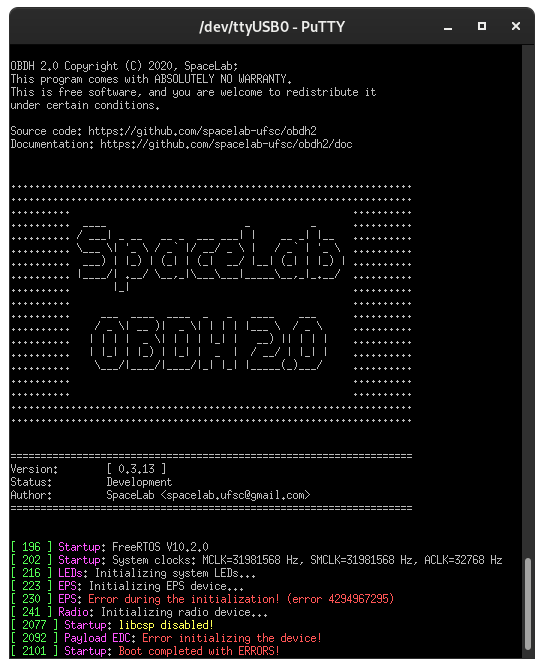
\includegraphics[width=0.75\textwidth]{figures/putty-output.png}
        \caption{Firmware initialization on PuTTy.}
        \label{fig:putty-output}
    \end{center}
\end{figure}

\section{Daughterboards Installation}

The daughterboard requirements might change for each application board attached. Then, it is important to check at least a minimal set of mandatory characteristics. First it is important to verify mechanical parameters that concerns to size (recommended $63.5 \times 43.5\ mm$), maximum height (no higher than $7\ mm$), screws attachment (refer to mechanical sheet \cite{obdh2-draftsman}) and contact connector positioning. After this, the electrical interface must be checked (refer to \autoref{sec:daughterboard-interface}). There are 3 different power supply options, a $3.3\ V$ source shared with the OBDH board itself, another $3.3\ V$ source shared with the antenna deployer, and the battery main bus that range from $5.4$ to $8.4\ V$. Lastly, depending on the application board design, it is necessary to check communication interfaces protocols and parameters, control inputs and outputs, and external interfaces with other modules.
